\documentclass[]{standalone}
%\usepackage{mathptmx}
%\renewcommand{\familydefault}{\rmdefault}
\usepackage[T1]{fontenc}
\usepackage[latin9]{inputenc}
\usepackage{siunitx}
\usepackage{array}
\usepackage{amsmath}
\usepackage{ifthen}
\usepackage{pgfplots}
\pgfplotsset{compat=1.14}
\usepackage{titling, graphicx}
\usepackage{tikz}
\usepackage{upgreek}
\usepackage{amsmath,amsthm}
\usepackage{strtikz}
\usetikzlibrary{shapes,arrows.meta,intersections,graphs,graphs.standard}
\usetikzlibrary{math,fit}
\usetikzlibrary{calc,intersections,through,backgrounds,decorations.pathmorphing}


\begin{document}
\begin{tikzpicture}
\dofs[startx = 0cm,
  starty = 0cm,
  dx = 1in,
  dy = 1cm,
  offset = 0.0cm,
  start angle = 110,
  end angle = 340,  
  radius = 1cm,
  xstring = $x$,
  ystring = $y$,  
  rstring = $\theta$,
  font size = \scriptsize,
  x location = left,
  y location = right,  
  r location = right,
  rotation=45]
\end{tikzpicture}
\end{document}